% !TEX root = VLDB-2026-DAGSmith-Dependency-Aware-Rewriting-for-dbt-Style-SQL-Pipelines.tex
% VLDB template version of 2020-08-03 enhances the ACM template, version 1.7.0:
% https://www.acm.org/publications/proceedings-template
% The ACM Latex guide provides further information about the ACM template

\documentclass[sigconf]{acmart}
%%
%% \BibTeX command to typeset BibTeX logo in the docs
\AtBeginDocument{%
  \providecommand\BibTeX{{%
    Bib\TeX}}}

\setcopyright{acmlicensed}
\copyrightyear{2027}
\acmYear{2027}
\acmDOI{XXXXXXX.XXXXXXX}
\acmConference[SIGMOD '27]{ACM SIGMOD International Conference on
  Management of Data}{June 13--19, 2027}{Huntington Beach, CA, USA}
\acmISBN{978-1-4503-XXXX-X/2027/06}


% !TEX root = VLDB-2026-DAGSmith-Dependency-Aware-Rewriting-for-dbt-Style-SQL-Pipelines.tex
\let\Bbbk\relax
\usepackage{amsmath,amssymb,mathtools}
\usepackage{algorithm}
\usepackage[noend]{algpseudocode}


% \usepackage[linesnumbered,ruled,vlined]{algorithm2e}
\usepackage{soul}
\usepackage{enumitem}
\usepackage{multirow} 
\usepackage{makecell}
\usepackage{subcaption}
\usepackage[page]{appendix}
\usepackage{graphicx}  % for \resizebox
\usepackage{hyperref}
\usepackage[nameinlink,capitalise]{cleveref}
\usepackage{listings}
\usepackage{framed}
\usepackage{xspace}
\usepackage{tikz}
\usetikzlibrary{arrows.meta, positioning, shapes.geometric, fit, calc, backgrounds}
\usepackage{xcolor}
\usepackage[normalem]{ulem}

% !TEX root = VLDB-2026-DAGSmith-Dependency-Aware-Rewriting-for-dbt-Style-SQL-Pipelines.tex
\captionsetup[figure]{font=small, labelfont=bf}

\newcommand{\cost}{\mathrm{cost}}
\newcommand{\pred}{\mathrm{pred}}
\newcommand{\override}[3]{#1\!\left[#2\leftarrow #3\right]}

\newcommand{\head}[1]{{{\vspace*{1mm} \noindent \textbf{#1.}}}}
\newcommand{\introhead}[1]{\noindent\textbf{#1 --}\enspace}


\newcommand{\tool}{{DAGSmith}\xspace}


\newfloat{listing}{htbp}{lol}
\floatname{listing}{Listing}


% Define a command for the internal figure headers
\newcommand{\figsubheader}[1]{%
    {\centering\small\textbf{#1}\par\medskip}%
}

\lstset{
    language=SQL,
    basicstyle=\tiny\ttfamily,
    % --- Keyword Highlighting ---
    keywordstyle=\color[HTML]{228B22}\bfseries, % Green for SQL keywords
    ndkeywordstyle=\color[HTML]{228B22}\bfseries,
    identifierstyle=\color{black},
    commentstyle=\color{gray},
    stringstyle=\color[HTML]{B22222},            % Dark red for strings like 's'
    % --- Other Settings ---
    numbers=left,
    numberstyle=\tiny\color{gray},
    stepnumber=1,
    numbersep=5pt,
    backgroundcolor=\color{gray!5},
    frame=single,
    rulecolor=\color{gray!40},
    breaklines=true,
    escapeinside={|}{|},
    showstringspaces=false,
    columns=flexible,
    xleftmargin=2mm
}


\definecolor{lin}{HTML}{e31a1c}
\newcommand{\linc}[1]{\textcolor{lin}{lin: #1}}


\raggedbottom

\settopmatter{authorsperrow=3}

\setcounter{topnumber}{3}
\setcounter{bottomnumber}{2}
\setcounter{totalnumber}{4}
\renewcommand{\topfraction}{0.9}
\renewcommand{\bottomfraction}{0.9}
\renewcommand{\textfraction}{0.07}
\renewcommand{\floatpagefraction}{0.85}

\AtBeginDocument{%
  \raggedbottom
  \setlength{\textfloatsep}{8pt plus 2pt minus 2pt}%     top/bottom float <-> text
  \setlength{\floatsep}{6pt plus 2pt minus 2pt}%         between two stacked floats
  \setlength{\intextsep}{8pt plus 2pt minus 2pt}%        around in-text [h] floats
  \setlength{\dbltextfloatsep}{10pt plus 2pt minus 2pt}% full-width float <-> text
}



\begin{document}

% \raggedbottom


\title{\tool: Dependency-Aware Rewriting for dbt-Style SQL Pipelines}

%%
%% The "author" command and its associated commands are used to define the authors and their affiliations.

\author{Anonymous authors}

\renewcommand{\shortauthors}{Anonymous Author(s)}


% \author{Jie Liu}
% \email{jiezzliu@umich.edu}
% \affiliation{%
%   \department{Computer Science and Engineering}
%   \institution{University of Michigan, Ann Arbor}
%   \country{USA}
% }

% \author{Lin Ma}
% \email{linmacse@umich.edu}
% \affiliation{%
%   \department{Computer Science and Engineering}
%   \institution{University of Michigan, Ann Arbor}
%   \country{USA}
% }

% \author{Barzan Mozafari}
% \email{mozafari@umich.edu}
% \affiliation{%
%   \department{Computer Science and Engineering}
%   \institution{University of Michigan, Ann Arbor}
%   \country{USA}
% }

% \renewcommand{\shortauthors}{Liu, Ma, and Mozafari}


% !TEX root = ../VLDB-2026-DAGSmith-Dependency-Aware-Rewriting-for-dbt-Style-SQL-Pipelines.tex
\begin{abstract}
Modern analytics is shifting from isolated, human-written SQL queries to large, recurring SQL programs produced and maintained by data teams, BI tools, and code-generation assistants. These programs increasingly appear as explicit dependency graphs of models, tasks, assets, and materialized tables. The graph makes inter-query dependencies visible, but database optimizers and most query rewriters still treat each SQL statement as the unit of optimization. This creates optimization opportunities that are invisible from inside one query: cross-boundary semantic reasoning, intermediate contract freedom, non-local semantic reuse, rewrite/materialization coupling, freshness-aware recomputation, and global composition of interacting rewrites.

We introduce \tool, a system for dependency-aware rewriting of dbt-style SQL pipelines. \tool treats a pipeline as a stable SQL pipeline DAG whose node definitions, dependency edges, output contracts, materialization choices, and refresh requirements are jointly available. It combines structural analysis over the DAG, LLM-guided refactoring, warehouse-backed equivalence checks, learned cost estimation, materialization tuning, frequency-aware scheduling, and global rewrite selection. \tool rewrites the structure around individual queries: factoring non-local shared work, pruning unused or mistimed computation, aligning refresh work with data-change and consumption rates, and selecting a globally consistent set of changes. This paper defines the optimization setting, identifies the opportunities created by explicit dependencies, and presents the architecture of \tool.
\end{abstract}


\begin{CCSXML}
<ccs2012>
 <concept>
  <concept_id>10002951.10002952.10003190.10003205</concept_id>
  <concept_desc>Information systems~Query optimization</concept_desc>
  <concept_significance>500</concept_significance>
 </concept>
 <concept>
  <concept_id>10002951.10002952.10003190.10003204</concept_id>
  <concept_desc>Information systems~Database query processing</concept_desc>
  <concept_significance>300</concept_significance>
 </concept>
 <concept>
  <concept_id>10002951.10003227.10003236.10003237</concept_id>
  <concept_desc>Information systems~Extraction, transformation and loading</concept_desc>
  <concept_significance>100</concept_significance>
 </concept>
 <concept>
  <concept_id>10010147.10010257</concept_id>
  <concept_desc>Computing methodologies~Machine learning</concept_desc>
  <concept_significance>100</concept_significance>
 </concept>
</ccs2012>
\end{CCSXML}
 
\ccsdesc[500]{Information systems~Query optimization}
\ccsdesc[300]{Information systems~Database query processing}
\ccsdesc[100]{Information systems~Extraction, transformation and loading}
\ccsdesc[100]{Computing methodologies~Machine learning}
 
% \keywords{SQL pipelines, query rewriting, dependency-aware optimization}



\maketitle



\section{Introduction}\label{sec:intro}

intro



% ============================================================
% Introductory motivating example, DAG-centric.
% Two DAG sketches (before/after) with four numbered annotations.
% ============================================================

% Required packages (in main.tex):
%   \usepackage{tikz}
%   \usetikzlibrary{positioning, arrows.meta, fit, calc, backgrounds}
%   \usepackage{xcolor}  % for the textcolor in source labels

\usetikzlibrary{positioning, arrows.meta, fit, calc, backgrounds}

\begin{figure*}[t]
\centering

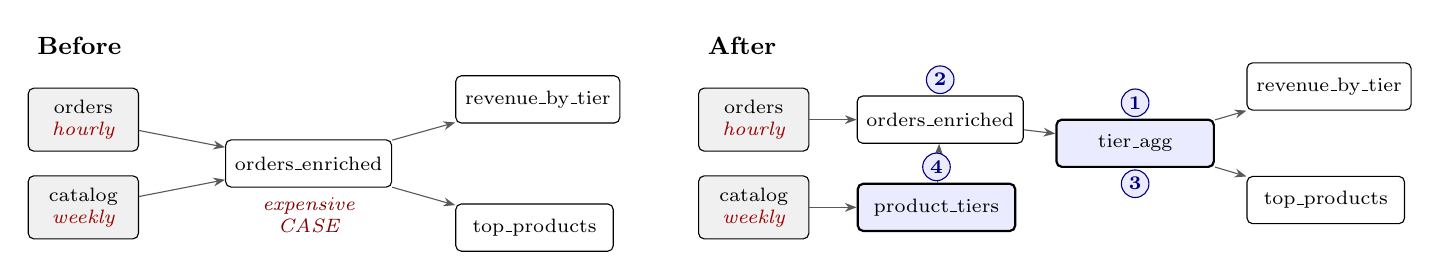
\begin{tikzpicture}[
  font=\small,
  node distance=5mm and 7mm,
  src/.style={draw, rounded corners=2pt, fill=gray!12,
              minimum width=14mm, minimum height=8mm,
              align=center, font=\scriptsize},
  model/.style={draw, rounded corners=2pt, fill=white,
                minimum width=20mm, minimum height=6mm,
                align=center, font=\scriptsize},
  newmodel/.style={draw, rounded corners=2pt, fill=blue!8, thick,
                   minimum width=20mm, minimum height=6mm,
                   align=center, font=\scriptsize},
  freq/.style={font=\scriptsize\itshape, color=red!60!black},
  edge/.style={-{Stealth[length=1.5mm]}, thin, gray!70!black},
  annot/.style={font=\scriptsize\bfseries, color=blue!50!black,
                draw=blue!50!black, circle, inner sep=0pt,
                minimum size=3.5mm, fill=blue!8},
]

% ------------------- BEFORE DAG (left half) -------------------
\node[font=\bfseries\small] (beforehdr) at (0,0) {Before};

\node[src, below=3mm of beforehdr.south west, anchor=north west] (orders0)
  {orders\\\textcolor{red!60!black}{\itshape hourly}};
\node[src, below=3mm of orders0] (catalog0)
  {catalog\\\textcolor{red!60!black}{\itshape weekly}};

\node[model, right=18mm of $(orders0)!0.5!(catalog0)$] (enr0) {orders\_enriched};
\node[model, above right=2mm and 8mm of enr0] (rev0) {revenue\_by\_tier};
\node[model, below right=2mm and 8mm of enr0] (top0) {top\_products};

\draw[edge] (orders0) -- (enr0);
\draw[edge] (catalog0) -- (enr0);
\draw[edge] (enr0) -- (rev0);
\draw[edge] (enr0) -- (top0);

% Callout: expensive CASE inside enr (motivates the moves)
\node[font=\scriptsize\itshape, color=red!50!black,
      below=0mm of enr0, align=center]
  {expensive\\CASE};

% ------------------- AFTER DAG (right half) -------------------
\node[font=\bfseries\small, right=72mm of beforehdr] (afterhdr) {After};

\node[src, below=3mm of afterhdr.south west, anchor=north west] (orders1)
  {orders\\\textcolor{red!60!black}{\itshape hourly}};
\node[src, below=3mm of orders1] (catalog1)
  {catalog\\\textcolor{red!60!black}{\itshape weekly}};

% New: product_tiers between catalog and enr (move 4)
\node[newmodel, right=6mm of catalog1] (ptiers1) {product\_tiers};

\node[model, right=6mm of orders1] (enr1) {orders\_enriched};

% New: tier_agg between enr and consumers (moves 1-3)
\node[newmodel, right=4mm of enr1, yshift=-3mm] (tagg1) {tier\_agg};

\node[model, above right=1mm and 4mm of tagg1] (rev1) {revenue\_by\_tier};
\node[model, below right=1mm and 4mm of tagg1] (top1) {top\_products};

\draw[edge] (orders1) -- (enr1);
\draw[edge] (catalog1) -- (ptiers1);
\draw[edge] (ptiers1) -- (enr1);
\draw[edge] (enr1) -- (tagg1);
\draw[edge] (tagg1) -- (rev1);
\draw[edge] (tagg1) -- (top1);

% --- Numbered annotations on the After DAG ---
% (1) factor: points at tier_agg
\node[annot] at ($(tagg1.north) + (0,2mm)$) (a1) {1};
% (2) drop columns: points at enr
\node[annot] at ($(enr1.north) + (0,2mm)$) (a2) {2};
% (3) materialization: points at tier_agg's interior
\node[annot] at ($(tagg1.south) + (0,-2mm)$) (a3) {3};
% (4) frequency split: points at product_tiers
\node[annot] at ($(ptiers1.north) + (0,2mm)$) (a4) {4};

\end{tikzpicture}

\vspace{2mm}

% --- Move legend below the DAGs ---
\begin{minipage}{0.97\textwidth}
\footnotesize
\begin{tabular}{@{}r@{\hspace{1.5mm}}p{0.92\textwidth}@{}}
\textbf{(1)} & \emph{Factor non-local shared work.} Both consumers group by \texttt{tier}; the optimizer extracts the shared aggregation into a new model invisible at any single SQL file. \\[0.5mm]
\textbf{(2)} & \emph{Equivalence is required at project outputs, not at every intermediate.} The optimizer can change an intermediate model in ways that no single-query rewriter would consider safe---e.g., narrowing its schema---as long as the project's leaf outputs are preserved. \\[0.5mm]
\textbf{(3)} & \emph{Refactoring and materialization are coupled.} The factorization in (1) is a win as a table and a wash as a view; refactoring decisions cannot be made without the materialization decision. \\[0.5mm]
\textbf{(4)} & \emph{Frequency is itself a structural dimension.} The expensive classification depends only on weekly data but lives inside an hourly model; splitting it onto the slow cadence requires a DAG rewrite invisible to per-execution cost. \\
\end{tabular}
\end{minipage}

\caption{An introductory walkthrough previewing the characteristics of dbt optimization addressed by \tool. The original DAG (\emph{Before}) has two sources at different update rates, an enriched intermediate, and two consumers; the whole pipeline runs hourly. \tool transforms it (\emph{After}) along four dimensions, summarized in the legend and addressed jointly in \S\ref{sec:approach}.}
\label{fig:intro-example}
\end{figure*}

\section{The dbt Optimization Setting}
\label{sec:motivating}

Before presenting our approach, we describe the optimization setting that \tool targets and illustrate, through three examples drawn from or inspired by real-world analytics pipelines, the kinds of cross-model optimizations that this setting enables but that fall outside the reach of existing techniques.

\subsection{What is a dbt Project?}
\label{sec:dbt-setting}

A dbt project is a directed acyclic graph (DAG) of SQL transformations, called \emph{models}.
Each model is a SQL transformation that produces a single output relation;
in this paper we focus on the standard \texttt{view} and \texttt{table} materialization modes.
Models reference one another through an explicit \texttt{ref()} construct that defines
the dependency edges of the DAG.
Each model is configured to be either \emph{materialized} as a physical table or
expanded inline as a \emph{view}.
The project is executed periodically against a target data warehouse:
when a model is run, dbt resolves its \texttt{ref()} calls, substitutes the appropriate
table reference or subquery, and submits the resulting SQL to the warehouse.

This setting differs from the workloads targeted by traditional query optimization in three ways that matter for our problem.

\head{Full DAG visibility}
The optimizer has access to the complete SQL definition of every model in the project, the dependency structure that connects them, and the materialization configuration of each model.
This is a stronger form of visibility than what is available to a database query optimizer, which rewrites one query at a time, or to multi-query optimization (MQO)~\cite{sellis1988multiple}, which sees a set of independent queries.
In both cases, the optimizer reasons over a flat collection of queries; in the dbt setting, it reasons over a dependency graph of transformations whose structure is itself under its control.
This shift in scope, from query rewriting to graph-level restructuring, is what makes optimizations such as merging, splitting, or inventing new intermediate models meaningful.

\head{Project stability}
A dbt project is a maintained software artifact, not an ad-hoc query workload.
It changes only when developers modify the underlying business logic or data model, not on every execution.
Between such changes, the same DAG is executed on a recurring schedule, often many times per day.
This stability justifies investing optimization effort that would not pay off in an online query processing setting: the cost of analysis (including potentially expensive cross-model reasoning) is amortized over many scheduled executions of the same DAG.

\head{Heterogeneous refresh patterns}
Different sources update at different rates, and different downstream consumers (dashboards, reports, downstream pipelines) require fresh results at different rates.
The refresh frequency of a model is therefore not a property of the model in isolation but is shaped by both its upstream sources and its downstream consumers.
Two consequences follow.
First, a model can sometimes be skipped entirely when its upstream inputs have not changed since the last run, so the effective cost of a model depends on how often it must actually be recomputed, not on how often the schedule fires.
Second, structural decisions about the DAG are not independent of refresh scheduling: splitting a model along a frequency boundary can move expensive computation onto a slower cadence, while merging two models can force the combined result to refresh at the rate of the faster input.
Optimizing the DAG therefore requires reasoning about structure and refresh rates jointly.
 
These three properties (visibility, stability, and frequency heterogeneity) together define a distinct optimization setting.
The optimizer is reasoning not about a query but about a \emph{program}: a stable DAG of SQL transformations whose structure, materialization, and refresh schedule are jointly under its control.
A real dbt project may contain hundreds of models, and the space of possible refactorings, materialization choices, and frequency-aware splits is far too large for developers to explore systematically by hand; this motivates the need for an automated optimizer rather than a guidebook of best practices.

\subsection{Motivating Examples}
\label{sec:motivating-examples}

We illustrate three classes of optimization that \tool discovers.
Each requires the optimizer to read and reason about SQL definitions \emph{across} model boundaries within the DAG, a capability that the dbt setting uniquely affords.
The SQL in each example is simplified for presentation; domain-specific details are abstracted away.

%==============================================================
% EXAMPLE 1: Semantic Factorization
%==============================================================
\head{Example 1: Cross-Model Semantic Factorization}
A pipeline contains seven classifier models that each tag orders with a service category (\texttt{dialysis}, \texttt{psychiatric}, and five others).
The input is a \texttt{claims} table in which each row represents one item of an order, so a single order has many rows.
Each classifier scans \texttt{claims}, keeps rows whose codes match its category's code list, and returns the distinct \texttt{order\_id}s of those rows.
The seven classifiers have \emph{different} SQL: different predicates, different code vocabularies, and in some cases different join structures.
Two representative classifiers are shown on the left of Figure~\ref{fig:ex-factorization}.


\begin{figure}[!htbp]
\begin{minipage}[t]{0.48\linewidth}
\figsubheader{Before: 7 classifiers (2 shown)}
\begin{lstlisting}[language=SQL]
-- dialysis_classifier
SELECT DISTINCT order_id
FROM {{ ref('claims') }}
WHERE bill_code LIKE '72%'
   OR taxonomy IN (set_dia_tax)
   OR diagnosis IN (set_dia_dx)


-- psychiatric_classifier
SELECT DISTINCT order_id
FROM {{ ref('claims') }}
WHERE revenue IN (set_psy_rev)
   OR diagnosis BETWEEN
        '290' AND '319'
\end{lstlisting}
\vspace{1.6\baselineskip}
\end{minipage}
\hfill
\begin{minipage}[t]{0.48\linewidth}
\figsubheader{After: precomputation+lookups}
\begin{lstlisting}[language=SQL]
-- order_flags (new)
SELECT order_id,
  MAX(CASE WHEN bill_code LIKE '72%'
    OR taxonomy IN (set_dia_tax)
    OR diagnosis IN (set_dia_dx)
    THEN 1 ELSE 0 END) AS f_dia,
  MAX(CASE WHEN ... 
    THEN 1 ELSE 0 END) AS f_psy,
  ...   -- 7 categories
FROM {{ ref('claims') }}
GROUP BY order_id
 
-- dialysis_classifier (rewritten)
SELECT order_id
FROM {{ ref('order_flags') }}
WHERE f_dia = 1
\end{lstlisting}
\end{minipage}
\caption{Cross-model semantic factorization. Seven classifiers with no syntactic overlap perform the same semantic operation on a shared parent. \tool synthesizes a new shared model that pre-aggregates all classifier flags in one pass.}
\label{fig:ex-factorization}
\end{figure}




The seven classifiers share no common subexpression, yet they all perform the same \emph{semantic operation}: for each order, decide whether any of its rows match a category-specific predicate.
\tool recognizes this cross-model pattern and factors it.
It synthesizes a new intermediate model \texttt{order\_flags} that, in a single pass over \texttt{claims}, computes one boolean flag per category by aggregating each category's predicate with \texttt{MAX(CASE WHEN ... THEN 1 ELSE 0 END)} grouped by \texttt{order\_id}.
Each original classifier is then rewritten as a lightweight lookup: select the orders whose corresponding flag in \texttt{order\_flags} is~$1$.
Seven full scans and seven independent grouping passes over \texttt{claims} are replaced with one pre-aggregation pass and seven inexpensive boolean filters.
 
This optimization requires three capabilities that go beyond traditional techniques.
First, the optimizer must recognize that seven syntactically dissimilar models perform the same semantic operation, which syntactic subexpression matching, the basis of multi-query optimization (MQO)~\cite{sellis1988multiple} and common subexpression elimination, cannot do.
Second, it must \emph{invent} a new intermediate model absent from the original project; materialized view recommendation tools~\cite{agrawal2000automated, bigsubs} synthesize candidate views, but they too rely on syntactic subexpression mining, of which the seven classifiers share none.
Third, it must rewrite the dependent models to consume the new intermediate while preserving end-to-end equivalence, a multi-model restructuring that single-query rewrite systems~\cite{wang2024wetune,zhou2024r} do not attempt.

%==============================================================
% EXAMPLE 2: Cross-Boundary Reasoning
%==============================================================
\head{Example 2: Cross-Boundary Semantic Reasoning}
The same project contains a classifier \texttt{nursing} that filters for skilled-nursing claims by facility code, then performs an anti-join against a sibling model \texttt{equipment} to exclude equipment-related claims (Figure~\ref{fig:ex-crossboundary}, left).
The anti-join forces the engine to materialize \texttt{equipment}, build a hash table, and probe it for every row of \texttt{claims}; it also introduces a DAG dependency that serializes the two models.



\begin{figure}[!htbp]
\begin{minipage}[t]{0.48\linewidth}
\figsubheader{Before: anti-join}
\begin{lstlisting}[language=SQL]
-- nursing
SELECT *
FROM {{ ref('claims') }} c
WHERE c.facility_code
        IN ('31','32')
  AND NOT EXISTS (
    SELECT 1
    FROM {{ ref('equipment') }} e
    WHERE e.order_id = c.order_id
      AND e.line_id  = c.line_id)
 
-- equipment (just a filter)
SELECT *
FROM {{ ref('claims') }}
WHERE category = 'equipment'
\end{lstlisting}
\end{minipage}
\hfill
\begin{minipage}[t]{0.48\linewidth}
\figsubheader{After: predicate}
\begin{lstlisting}[language=SQL]
-- nursing (rewritten)
SELECT *
FROM {{ ref('claims') }} c
WHERE c.facility_code
        IN ('31','32')
  AND (c.category IS NULL
    OR c.category <> 'equipment')


 
-- equipment is removed if no
-- other model depends on it;
-- otherwise its definition
-- is unchanged.
\end{lstlisting}
\vspace{1.6\baselineskip}
\end{minipage}
\caption{Cross-boundary semantic reasoning. By reading the SQL of the sibling \texttt{equipment} model, \tool determines that the anti-join is equivalent to a scalar predicate on a shared parent. The hash anti-join, the auxiliary scan, and the DAG dependency are all eliminated.}
\label{fig:ex-crossboundary}
\end{figure}




By reading the SQL definition of \texttt{equipment}, \tool discovers that it computes nothing more than a single-predicate filter on a shared parent.
The anti-join is therefore equivalent to an inline scalar predicate on \texttt{claims}, as shown on the right of the figure: the hash anti-join, the auxiliary scan, and the cross-model DAG dependency are all eliminated.
The same reasoning generalizes to every sibling classifier that uses \texttt{equipment} as an exclusion list, compounding the benefit across the pipeline.

The equivalence enabling this rewrite is not declared anywhere; it is \emph{embedded in the SQL of another model file}.
A traditional engine sees \texttt{equipment} either as a base table to be probed or as a view to be expanded into the local query, neither of which performs the cross-model analysis needed to eliminate the join entirely.
We acknowledge a tradeoff: the rewrite couples \texttt{nursing} to the current definition of \texttt{equipment}, so a future change to that definition would require updating the rewritten consumers.
In practice, stable upstream models such as \texttt{equipment} change rarely, and \tool re-evaluates the project after each developer change, so the cost of re-deriving the rewrite is amortized over many executions.

%==============================================================
% EXAMPLE 3: Frequency-Aware
%==============================================================
\head{Example 3: Frequency-Aware Restructuring}
Different sources in a dbt project update at different rates, and the structure of the DAG determines how much computation must be repeated at each high-frequency refresh.
Consider a model that joins fast-changing transactional data with slow-changing reference data and applies expensive classification logic to the slow-changing side (Figure~\ref{fig:ex-frequency}, left).


\begin{figure}[!htbp]
\begin{minipage}[t]{0.48\linewidth}
\figsubheader{Before: hourly classification}
\begin{lstlisting}[language=SQL]
-- order_summary  (hourly)
SELECT o.order_id, o.amount,
  CASE
    WHEN p.code IN (set_A) THEN 'A'
    WHEN p.code IN (set_B) THEN 'B'
    ...
  END AS category
FROM {{ ref('orders') }}  o
JOIN {{ ref('catalog') }} p
  ON o.product_id = p.product_id

  
-- orders:  hourly
-- catalog: weekly
\end{lstlisting}
\vspace{1.6\baselineskip}
\end{minipage}
\hfill
\begin{minipage}[t]{0.48\linewidth}
\figsubheader{After: split by frequency}
\begin{lstlisting}[language=SQL]
-- product_categories (weekly)
SELECT product_id,
  CASE
    WHEN code IN (set_A) THEN 'A'
    WHEN code IN (set_B) THEN 'B'
    ...
  END AS category
FROM {{ ref('catalog') }}
 
-- order_summary (hourly)
SELECT o.order_id, o.amount,
       pc.category
FROM {{ ref('orders') }} o
JOIN {{ ref('product_categories') }} pc
  USING (product_id)
\end{lstlisting}
\end{minipage}
\caption{Frequency-aware restructuring. Splitting the model along the frequency boundary moves expensive classification onto a weekly cadence; the hourly model becomes a lightweight join.}
\label{fig:ex-frequency}
\end{figure}


Because \texttt{orders} changes hourly, \texttt{order\_summary} re-executes hourly, and the multi-branch classification over \texttt{catalog} is recomputed on every hourly refresh, despite its inputs changing only weekly.
\tool traces the update frequency from each source through the DAG, identifies that this model has \emph{mixed-frequency inputs}, and splits it along the frequency boundary.
The expensive classification is extracted into a new slow-frequency model, and the original model becomes a lightweight equi-join.
When this pattern recurs across many consumers of the same slow-changing reference data, the savings compound: each hourly refresh avoids redundant recomputation of logic whose inputs have not changed.

This optimization is invisible to optimizers that treat cost as a fixed per-query quantity: the benefit of splitting the model is realized only when the two halves are known to execute at different rates.
Materialized view selection considers update cost but does not restructure the DAG to align computation with update frequency, and traditional query rewriters have no notion of refresh schedule at all.

\subsection{Why Existing Techniques Fall Short}
\label{sec:why-different}

The three examples above are not isolated curiosities; they illustrate a general capability gap.
Single-query rewrite systems~\cite{wang2024wetune,zhou2024r,chakravarthy1990logic} operate within the boundary of one query and cannot restructure across model files.
Multi-query optimization and common subexpression elimination~\cite{sellis1988multiple} share intermediate computations across queries but rely on syntactic matching, so they miss the cross-model semantic equivalence in Example~1.
Materialized view selection~\cite{agrawal2000automated} chooses among existing view candidates and treats update cost as a static parameter rather than as a structural driver of DAG design (Example~3).
Code clone detection and lineage tools can identify structural similarity or trace data provenance, but they do not perform the optimization itself.

The gap is not that any one of these techniques is poorly designed; it is that none of them targets the setting we are concerned with.
Optimizing a dbt project requires (1) cross-model semantic analysis, (2) DAG-aware structural rewriting that may invent or merge models, and (3) frequency-aware reasoning that ties structural decisions to update rates.
The remainder of this paper presents an approach that integrates these three capabilities into a coherent optimization framework.






\begin{comment}
    


\begin{figure}[t]
\figsubheader{Before: 7 independent classifiers (2 shown)}
% \centering\textbf{Before: 7 independent classifiers (2 shown)}
\begin{lstlisting}[language=SQL]
-- dialysis_classifier
SELECT DISTINCT order_id
FROM {{ ref('claims') }}
WHERE bill_code LIKE '72%'
   OR taxonomy IN (set_dialysis_tax)
   OR diagnosis IN (set_dialysis_dx)

-- psychiatric_classifier
SELECT DISTINCT order_id
FROM {{ ref('claims') }}
WHERE revenue IN (set_psych_rev)
   OR diagnosis BETWEEN '290' AND '319'
\end{lstlisting}

\figsubheader{After: shared pre-aggregation + lookups}
% \centering\textbf{After: shared pre-aggregation + lookups}
\begin{lstlisting}[language=SQL]
-- order_flags  (new shared model)
SELECT order_id,
  MAX(CASE WHEN bill_code LIKE '72%'
        OR taxonomy IN (set_dialysis_tax)
        OR diagnosis IN (set_dialysis_dx)
       THEN 1 ELSE 0 END) AS f_dialysis,
  MAX(CASE WHEN ... THEN 1 ELSE 0 END) AS f_psych,
  ...  -- flags for all 7 categories
FROM {{ ref('claims') }}
GROUP BY order_id

-- dialysis_classifier (rewritten)
SELECT order_id FROM {{ ref('order_flags') }}
WHERE f_dialysis = 1
\end{lstlisting}
\caption{Cross-model semantic factorization. Seven classifiers with no syntactic overlap perform the same semantic operation on a shared parent. \tool synthesizes a new shared model that pre-aggregates all classifier flags in one pass.}
\label{fig:ex-factorization}
\end{figure}

=========================




\begin{figure}[t]
\figsubheader{Before: anti-join against sibling model}
% \centering\textbf{Before: anti-join against sibling model}
\begin{lstlisting}[language=SQL]
-- nursing
SELECT *
FROM {{ ref('claims') }} c
WHERE c.facility_code IN ('31','32')
  AND NOT EXISTS (
    SELECT 1
    FROM {{ ref('equipment') }} e
    WHERE e.order_id = c.order_id
      AND e.line_id  = c.line_id)

-- equipment  (definition is just a filter)
SELECT * FROM {{ ref('claims') }}
WHERE category = 'equipment'
\end{lstlisting}

\figsubheader{After: anti-join replaced with predicate}
% \centering\textbf{After: anti-join replaced with predicate}
\begin{lstlisting}[language=SQL]
-- nursing  (rewritten)
SELECT *
FROM {{ ref('claims') }} c
WHERE c.facility_code IN ('31','32')
  AND (c.category IS NULL
    OR c.category <> 'equipment')

-- equipment is removed if no other model
-- depends on it; otherwise its definition
-- is unchanged.
\end{lstlisting}
\caption{Cross-boundary semantic reasoning. By reading the SQL of the sibling \texttt{equipment} model, \tool determines that the anti-join is equivalent to a scalar predicate on a shared parent. The hash anti-join, the auxiliary scan, and the DAG dependency are all eliminated.}
\label{fig:ex-crossboundary}
\end{figure}



=========================



\begin{figure}[t]
\figsubheader{Before: classification re-runs hourly}
% \centering\textbf{Before: classification re-runs hourly}
\begin{lstlisting}[language=SQL]
-- order_summary  (runs hourly)
SELECT o.order_id, o.amount,
  CASE
    WHEN p.code IN (set_A) THEN 'A'
    WHEN p.code IN (set_B) THEN 'B'
    ...
  END AS category
FROM {{ ref('orders') }}  o   -- hourly
JOIN {{ ref('catalog') }} p   -- weekly
  ON o.product_id = p.product_id
\end{lstlisting}

\figsubheader{After: split along frequency boundary}
% \centering\textbf{After: split along frequency boundary}
\begin{lstlisting}[language=SQL]
-- product_categories  (new, runs weekly)
SELECT product_id,
  CASE
    WHEN code IN (set_A) THEN 'A'
    WHEN code IN (set_B) THEN 'B'
    ...
  END AS category
FROM {{ ref('catalog') }}

-- order_summary  (rewritten, hourly, lightweight)
SELECT o.order_id, o.amount, pc.category
FROM {{ ref('orders') }} o
JOIN {{ ref('product_categories') }} pc
  USING (product_id)
\end{lstlisting}
\caption{Frequency-aware restructuring. Splitting the model along the frequency boundary moves expensive classification onto a weekly cadence; the hourly model becomes a lightweight join.}
\label{fig:ex-frequency}
\end{figure}









\end{comment}
% !TEX root = ../VLDB-2026-DAGSmith-Dependency-Aware-Rewriting-for-dbt-Style-SQL-Pipelines.tex
\section{Approach}
\label{sec:approach}

% Required preamble (in main.tex):
%   \usepackage{tikz}
% This file loads its own TikZ libraries below, so no \usetikzlibrary
% is needed in main.tex on its account.

\usetikzlibrary{arrows.meta, positioning, shapes.geometric, fit, calc}

\begin{figure*}[t]
\centering
\resizebox{\textwidth}{!}{%
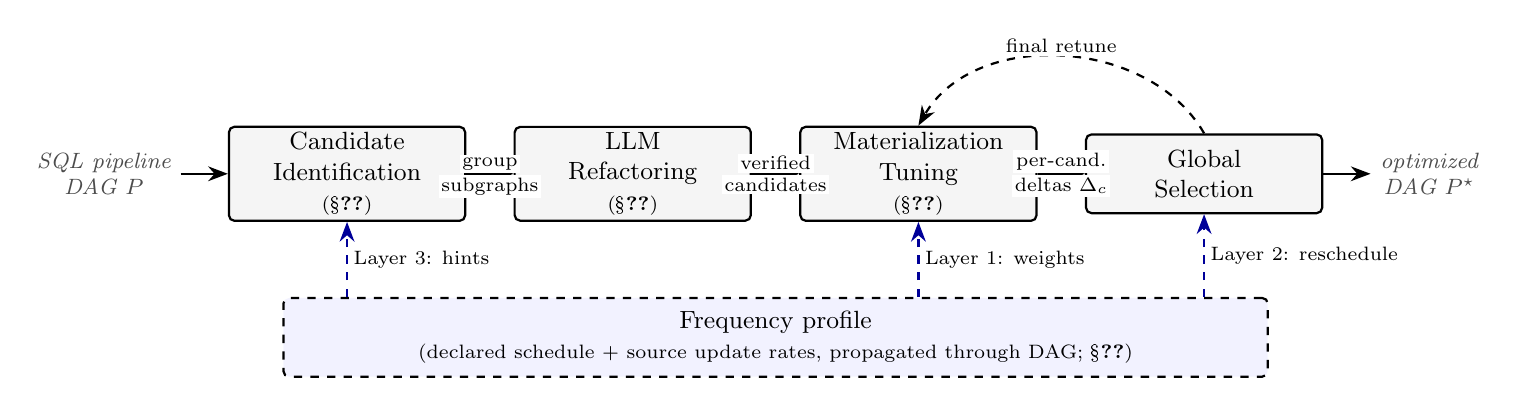
\begin{tikzpicture}[
    font=\small,
    node distance=4mm and 6mm,
    stage/.style={
        draw, rounded corners=2pt, thick,
        minimum height=10mm, minimum width=30mm,
        align=center, fill=black!4,
        inner sep=2pt
    },
    freqstage/.style={
        draw, rounded corners=2pt, thick, dashed,
        minimum height=4mm, minimum width=28mm,
        align=center, fill=blue!5,
        inner sep=2pt
    },
    io/.style={
        align=center, font=\footnotesize\itshape, text=black!70
    },
    arrow/.style={
        -{Stealth[length=2.5mm]}, thick
    },
    freqarrow/.style={
        -{Stealth[length=2.5mm]}, thick, dashed, draw=blue!60!black
    },
    arrowlabel/.style={
        font=\scriptsize, midway, fill=white, inner sep=1pt
    }
]

% --- input ---
\node[io] (input) {SQL pipeline\\DAG $P$};

% --- four pipeline stages, left to right ---
\node[stage, right=of input] (s1) {Candidate\\Identification\\\scriptsize(\S\ref{sec:candidate-identification})};
\node[stage, right=of s1]    (s2) {LLM\\Refactoring\\\scriptsize(\S\ref{sec:llm-refactoring})};
\node[stage, right=of s2]    (s3) {Materialization\\Tuning\\\scriptsize(\S\ref{sec:materialization})};
\node[stage, right=of s3]    (s4) {Global\\Selection};

% --- output ---
\node[io, right=of s4] (output) {optimized\\DAG $P^\star$};

% --- main pipeline arrows with artifact labels ---
\draw[arrow] (input) -- (s1);
\draw[arrow] (s1) -- node[arrowlabel, above]{group} node[arrowlabel, below]{subgraphs} (s2);
\draw[arrow] (s2) -- node[arrowlabel, above]{verified} node[arrowlabel, below]{candidates} (s3);
\draw[arrow] (s3) -- node[arrowlabel, above]{per-cand.} node[arrowlabel, below]{deltas $\Delta_c$} (s4);
\draw[arrow] (s4) -- (output);

% --- frequency profile band: one wide box spanning under stages s1-s4 ---
\node[freqstage, below=2mm of s2.south,
      minimum width=125mm, minimum height=10mm,
      anchor=north] (fband)
  at ($(s1.south west)!0.5!(s4.south east) + (0,-8mm)$)
  {Frequency profile\\\scriptsize(declared schedule + source update rates,
   propagated through DAG; \S\ref{sec:frequency})};

% Frequency arrows: profile feeds the three stages it touches, each labeled by layer
\draw[freqarrow] (fband.north -| s1.south) -- (s1.south)
  node[arrowlabel, right=1pt, fill=white]{\scriptsize Layer 3: hints};
\draw[freqarrow] (fband.north -| s3.south) -- (s3.south)
  node[arrowlabel, right=1pt, fill=white]{\scriptsize Layer 1: weights};
\draw[freqarrow] (fband.north -| s4.south) -- (s4.south)
  node[arrowlabel, right=1pt, fill=white]{\scriptsize Layer 2: reschedule};

% Final tuning loop-back: after selection, retune materialization on combined DAG
\draw[arrow, dashed]
  (s4.north) to[out=120, in=60]
  node[arrowlabel, above, fill=white]{final retune}
  (s3.north);

\end{tikzpicture}%
}
\caption{End-to-end pipeline of \tool. The top row shows the four main stages and the artifacts that flow between them; after global selection, a final materialization pass retunes the combined DAG. The dashed band underneath is the frequency-aware overlay (\S\ref{sec:frequency}): a single frequency profile feeds three of the four stages, contributing structural splitting hints, cost weights for materialization tuning, and schedule corrections at selection.}
\label{fig:pipeline}
\end{figure*}


\linc{Okay in general, I think this section has way too many implementation details and less intuitive lessons. The purpose of a paper is not to document every details of the implementation so that others will recreate every single step. You'll have your code released and they can reference your code anyway. Rather, the purpose is do convery what are the key technical challenges to solve this problem, (intuitively) what are our solutions to solve these challenges and why we choose these solutions, and what lessons did we learn. Implementaiton details are helpful only if we have the space and if that supports our argument for the solution. But having too many can be distracting. I also think having 5 subsections (components) are a bit too many. I would suggest having only 3-4 subsections. (I think earlier you wrote there are 3 optimization dimensions? That might be a good breakdown for the subsections. It seems that in the ablation study you only categorize three optimizations anyway.) And within each subsection, you start with what technical challenges you're going to solve (and why such challenges exist in our problem), and intuitively how your solution works (and why it solves the challenges). A figure illustrating the sollution would be a plus. Then, you go into a little bit of details to just have the audience have a slighly deeper understanding. You can take a look at other papers (or even your previous papers) to see how long this should be. Readers/Reviewers won't appreciate if you add too many details and they couldn't easily get the big picture.}

\tool{} optimizes a SQL pipeline DAG along three interacting dimensions: graph refactoring, materialization, and refresh frequency. \linc{I know Barzan is still reorganizing sections 0-2, but since we have three dimensions here, we know just condense the earlier six opportunites to three, and we have an optimization for each of the opportunity? We can probably connect each of the example in Section 2 to one dimension here as well. Wouldn't this be much more succinct and saving lots of space?} These are the same three dimensions our evaluation ablates, and each corresponds to the opportunities of Section~2: refactoring restructures the DAG to share or remove work (Examples~1 and~2), materialization decides which results are persisted, and frequency aligns each node's execution rate with how often its inputs change (Example~3). They cannot be decided independently. 

% The benefit of a refactoring depends on which nodes are materialized, the best materialization configuration depends on the structure of the DAG, and both depend on how often each node executes. A pipeline with hundreds or thousands of models admits an enormous space of candidate refactorings, materialization assignments, and refresh schedules; exhaustive search is infeasible, and optimizing the three dimensions in separate passes misses these interactions and produces decisions that conflict at the boundaries.

\linc{I think we need to reference Figure 5 at the beginning of this paragraph} \tool{} realizes these dimensions in the pipeline of Figure~\ref{fig:pipeline}. Cheap structural analyses first scan the whole DAG and rank model groups by a fingerprint-based score that estimates the benefit of refactoring them jointly (Section~\ref{sec:candidate-identification}). The top-ranked groups are passed to an LLM, which reasons over each region and proposes one or more concrete refactorings (Section~\ref{sec:llm-refactoring}). 
The structural analyses decide where in the DAG to refactor; the LLM decides what refactoring to perform. \linc{Since we mentioned LLM, I think we need to add one sentence to talk about the correctness guarantee. Otherwise, I think that would be the first question that the reviewer raises.} Every refactoring is adopted only after it passes equivalence checks that the LLM writes for itself and that are tested against the project's real data. A refactoring's benefit depends on how its nodes are materialized, so \tool{} tunes each candidate's materialization with a learned cost model and selects a compatible subset to adopt (Section~\ref{sec:materialization}). The frequency dimension cuts across these stages (Section~\ref{sec:frequency}): it reweights the cost-driven decisions, removes refreshes that recompute unchanged data, and contributes structural splitting candidates to the first stage.





% % Required preamble (add to main.tex if not already there):
% % \usepackage{algorithm}
% % \usepackage{algpseudocode}

% \begin{algorithm}[t]
% \caption{\tool{} optimization pipeline.}
% \label{alg:pipeline}
% \begin{algorithmic}[1]
% \Require SQL pipeline DAG $P$, frequency profile $\Phi$
% \Ensure optimized DAG $P^\star$
% \State $f \gets \textsc{PropagateFrequencies}(P, \Phi)$
% \State $\mathcal{G} \gets \textsc{ReuseAnalysis}(P) \cup \textsc{PruneAnalysis}(P)$
% \Statex \hspace{3.6em} $\cup\ \textsc{FrequencySplitHints}(P, f)$ \Comment{\S\ref{sec:candidate-identification}}
% \State $\mathcal{C} \gets \textsc{LLMRefactor}(\mathcal{G}, P)$ \Comment{\S\ref{sec:llm-refactoring}}
% \State $\delta_{\text{orig}} \gets \textsc{MaterializationTune}(P, f)$ \Comment{\S\ref{sec:materialization}}
% \ForAll{$c \in \mathcal{C}$}
%   \State $P_c \gets \textsc{Apply}(P, c)$
%   \State $\Delta_c \gets \delta_{\text{orig}} - \textsc{MaterializationTune}(P_c, f)$
% \EndFor
% \State $H \gets \textsc{ConflictGraph}(\mathcal{C})$
% \State $\mathcal{C}^\star \gets \textsc{SelectILP}(\mathcal{C}, \{\Delta_c\}, H)$ \Comment{\S\ref{sec:materialization}}
% \State $P^\star \gets \textsc{Apply}(P, \mathcal{C}^\star)$
% \State $\textsc{MaterializationTune}(P^\star, f)$ \Comment{final retune}
% \State \Return $\textsc{ReconcileSchedule}(P^\star, f)$ \Comment{\S\ref{sec:frequency}}
% \end{algorithmic}
% \end{algorithm}


\subsection{Candidate Identification}
\label{sec:candidate-identification}

\linc{I don't think we have established why we want to use LLM for refactoring yet. So I think either you have to establish that here, or just talk about refactoring is costly in general, without specifically emphasizing LLMs.}
Deciding how to refactor a region of the pipeline requires reasoning about what its models compute, a semantic judgment beyond the reach of syntactic rewrite rules, so \tool{} delegates it to an LLM. A project with hundreds of models admits an enormous number of conceivable refactorings, and running the LLM on every model group would be both prohibitively expensive and dominated by trivial proposals. \tool{} therefore divides the labor: cheap structural analyses scan the whole DAG and surface the few regions where a refactoring is likely to pay off, and the expensive LLM reasoning is reserved for those regions.

\linc{Before getting into all the details below, I think it would be good to have one paragraph to discuss intuitively how your analysis works and what it achieves (if you can pair that with a figure, that's even better). The rest of this subsection is just implementation details. If intuitively the method makes sense, we would be good. We can either keep the details below or just condense them if we're short on space.}

At its core the analysis must decide when two models do the same expensive work, and the obvious tests miss real cases. Matching SQL text fails on any rephrasing. Matching plan structure is stronger, since multi-query optimization and view-matching already handle join order, predicate order, and aliasing, but they still miss equivalences that change the plan's shape, and they see only one compiled query at a time. In Figure~\ref{fig:dataflow-grouping}, Models A and B are equivalent but apply a filter on opposite sides of the \textsc{group by}, so a structural matcher sees two different trees. \tool{} instead matches on what each model computes, independent of how the SQL is written and of where the model sits in the DAG, so the two models reduce to one candidate that the LLM and an equivalence check then confirm is safe to share. Two analyses do this: \emph{reuse} finds repeated expensive work to share, and \emph{prune} finds work that no downstream model consumes or that runs too early. Only the highest-scoring regions go to the LLM.
 
\begin{figure}[t]
\centering
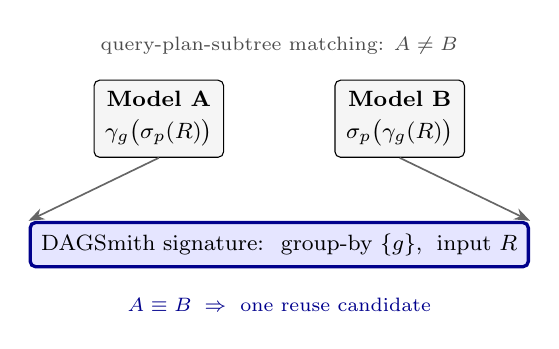
\begin{tikzpicture}[
  font=\small,
  >={Stealth[length=2mm]},
  q/.style={draw, rounded corners=2pt, align=center, fill=black!4, inner sep=4pt, font=\footnotesize},
  canon/.style={draw=blue!55!black, very thick, rounded corners=2pt, align=center, fill=blue!10, inner sep=4pt, font=\footnotesize},
  arr/.style={->, semithick, draw=black!60},
  lbl/.style={font=\scriptsize, text=black!70}
]
\node[q] (A) {\textbf{Model A}\\[2pt]$\gamma_{g}\bigl(\sigma_{p}(R)\bigr)$};
\node[q, right=14mm of A] (B) {\textbf{Model B}\\[2pt]$\sigma_{p}\bigl(\gamma_{g}(R)\bigr)$};
% verdict placed just above the boxes
\node[lbl, anchor=south] (neq) at ($(A.north)!0.5!(B.north)+(0,2mm)$)
  {query-plan-subtree matching: $A \neq B$};
% signature just below the boxes
\node[canon, anchor=north] (C) at ($(A.south)!0.5!(B.south)+(0,-8mm)$)
  {\tool{} signature:\; group-by $\{g\}$,\; input $R$};
\draw[arr] (A.south) -- (C.north west);
\draw[arr] (B.south) -- (C.north east);
\node[lbl, text=blue!55!black, below=2.5mm of C] {$A \equiv B \;\Rightarrow\;$ one reuse candidate};
\end{tikzpicture}
\caption{Candidate identification matches on computation, not on plan shape. Models A and B are equivalent (the filter is on the grouping key) but apply it on opposite sides of the \textsc{group by}, so plan-subtree matching sees two trees, while \tool{} reduces both to one signature and a single reuse candidate.}
\label{fig:dataflow-grouping}
\end{figure}

\head{Dataflow representation}
Both analyses run on a \emph{dataflow representation} that \tool{} builds for each model: its SQL compiled into a tree of typed operators, with every column resolved back through the chain of models that produced it via the project's \texttt{ref()} graph. Models A and B of Figure~\ref{fig:dataflow-grouping} are shown in this form, each applying a filter and a group-by to an input $R$; resolving the columns shows that both group $R$ by the same key $g$, whatever the surrounding SQL looks like and wherever the two models sit in the DAG. The analyses read this representation rather than the SQL text.

\head{Reuse analysis}
Reuse analysis summarizes each model by a signature of its expensive operations (joins and group-by aggregations), their keys, and their resolved inputs, then groups models whose signatures match. A high reuse score is a \emph{targeting signal}, not an instruction to materialize a shared subexpression: it marks where the LLM should look.

\head{Prune analysis}
Prune analysis targets joins, in two forms. A \emph{redundant} join produces a result that no downstream model consumes, confirmed by tracing column lineage from the leaf models; it can be removed outright, and a semi-join collapses to a predicate when its filtering set is already derivable from columns in the probed relation. A \emph{mistimed} join is semantically correct but computed too early: when one side feeds expensive downstream operations whose results do not depend on the other side's columns, pushing the join past those operations avoids carrying its product through them. Prune analysis also flags unused projected columns whose removal simplifies upstream definitions. What sets this apart from local dead-code elimination is its scope: whether a join's result is used, or used too soon, is a fact about the rest of the pipeline that a single-query rewriter cannot see.

\head{From candidates to subgraphs}
The two analyses produce a ranked stream of candidate model groups. For each, \tool{} extracts a subgraph containing the candidate models plus a configurable neighborhood of upstream and downstream context, enough for the LLM to reason about correctness; groups whose neighborhoods exceed the bound are skipped. The next subsection describes how the LLM turns these subgraphs into concrete refactorings.




\subsection{LLM Refactoring}
\label{sec:llm-refactoring}

\linc{Well, why do we want to use an LLM to do this in the first place? We either have to establish this earlier or justify it here.}
As motivated in the overview, producing these cross-boundary, semantic rewrites is a reasoning task rather than a pattern-matching one, which is why \tool{} uses an LLM rather than a fixed rule set. But asking an LLM to rewrite SQL that will run against a production warehouse raises three problems: the rewrite may be \emph{slower} than the original, may be \emph{incorrect}, or may be \emph{too expensive to generate} when a region contains many models. The challenge for this stage is to obtain useful rewrites while controlling all three risks.

\linc{Similarly, I think one paragraph to discuss intuitively how your approach works and what it achieves (better with a figure) can be valuable. The details can be reduce.}
\tool{} controls these risks by refusing to treat rewriting as a single LLM call. It splits the work into four roles, each a separate call with one job: a \emph{proposer} reads the region and lists candidate optimizations, an adversarial \emph{critic} rejects proposals that would slow the pipeline or silently change its results, a \emph{rewriter} turns the survivors into concrete SQL, and a \emph{verifier} tests each rewrite against the warehouse's real data before it is trusted. Separating proposal from criticism keeps a single prompt from having to be both creative and skeptical, and grounding acceptance in real data rather than in the model's own assurance is what makes adopting LLM-written SQL safe. A fifth, lighter mechanism propagates an accepted rewrite across near-duplicate models, so the four-call sequence need not run on each one.

\head{Proposal}
The first call ingests the subgraph's SQL and dependency edges and produces a domain-level reading of the region: a short semantic summary of each model and the end-to-end business question the subgraph answers. This reading is what lets later stages recognize equivalent computations written in dissimilar SQL. Its output is a list of \emph{opportunities}, each naming the work it would remove or shrink and the mechanism by which it would do so; opportunities are proposals, not yet rewrites.

\head{Filtering}
A second call acts as an adversarial critic over the proposals. The separation is deliberate: a single LLM asked at once to propose and to doubt does neither well, with proposal mode dominating. The critic catches both slowdowns and correctness traps. A slowdown is, for instance, a proposal that looks like reuse-driven savings but adds a write and a scan without reducing downstream work. A correctness trap is shown in Figure~\ref{fig:critic-catch}: the proposal drops a join by reading a tag from a sibling that has been deduplicated to one row per item, silently discarding the secondary tags the original join admitted. The critic returns one of three verdicts, \emph{approve}, \emph{reject}, or \emph{conditional}; a conditional verdict records a data property the rewrite must hold to, which is carried into the next stage.

\begin{figure}[!htbp]
\begin{minipage}[t]{0.48\linewidth}
\figsubheader{Original: join admits all tags}
\begin{lstlisting}[language=SQL]
SELECT i.item_id,
  MAX(CASE WHEN t.tag='A'
    THEN 1 ELSE 0 END) AS flag_a
FROM {{ ref('items') }} i
JOIN {{ ref('item_tags') }} t
  USING (item_id)
GROUP BY i.item_id
\end{lstlisting}
\end{minipage}
\hfill
\begin{minipage}[t]{0.48\linewidth}
\figsubheader{Proposal: drop join, read tag}
\begin{lstlisting}[language=SQL]
SELECT s.item_id,
  CASE WHEN s.tag='A'
    THEN 1 ELSE 0 END AS flag_a
FROM {{ ref('items_staged') }} s
-- items_staged keeps one tag/item;
-- secondary tags are silently lost
\end{lstlisting}
\end{minipage}
\caption{Correctness trap rejected by the proposal critic. The original aggregates over all tags per item; the proposal reads from a sibling that has been deduplicated to one tag per item, and silently drops the rest.}
\label{fig:critic-catch}
\end{figure}

\head{Rewriting}
The opportunities that survive filtering, together with the analysis and the SQL of the affected nodes, go to a third call that produces concrete refactored SQL: it may rewrite nodes, mark nodes as removed, or introduce new shared nodes. Conditional opportunities carry their recorded constraints into this prompt. A node with consumers outside the subgraph may be rewritten internally but must produce identical output rows, since its contract with those consumers is fixed.

\head{Equivalence verification}
A rewrite that passed filtering can still change the data, especially when one bundles several opportunities and a trap rejected on its own reappears nested inside a larger change: the staged-input shortcut of Figure~\ref{fig:critic-catch}, for instance, can resurface inside a consolidated aggregation the critic approved on other grounds. \tool{} therefore treats equivalence as an empirical question against real data. A fourth call, the \emph{correctness critic}, states for each adopted opportunity the data invariant that must hold for the rewrite to be safe and renders it as a SQL diagnostic that returns zero rows when the invariant holds and rows when it is violated. The diagnostics run against the target warehouse under a per-query byte cap; any returned row is a counterexample drawn from real data. Failed invariants are appended to the rewriting prompt, and the LLM must either find a distinctly different strategy that respects them or restore the original logic. The loop ends when the rewrite passes all diagnostics, the LLM reports no further distinct strategy, or a per-group attempt budget is exhausted, in which case the group reverts to its original SQL and contributes no candidate.

\head{Model families and propagation}
A single subgraph often contains many near-duplicate models that apply the same operation to different data subsets. The proposal stage identifies such a group, designates one \emph{representative}, and records how the other members differ; only the representative runs through the four calls above, after which a lighter per-member call applies the same change in parallel. This is a scalability mechanism for projects whose models exhibit family structure; where there is none, the family map collapses to singletons and the main sequence simply runs over every model.


\subsection{Materialization Tuning}
\label{sec:materialization}

A refactoring has no benefit that can be read off in isolation. Whether it helps depends on which of its nodes are stored as tables and which are inlined as views, the best choice differs from one candidate to the next, and the choice is non-local: inlining one node changes the predicted cost of every node downstream of it. \tool{} therefore scores every candidate under its own best materialization assignment, with the unrefactored DAG included as a candidate and serving as the baseline. A second challenge arises once the candidates are scored: they overlap, so two refactorings can touch the same model and cannot both be adopted, and the chosen ones must be composed into a single project rather than taken all at once. This subsection covers both, finding a candidate's best materialization and then selecting a compatible set.

\head{Cost of a DAG configuration}
Given a materialization assignment, the pipeline's cost is computed in one topological pass. A table pays its own predicted slot time once per execution and exposes its predicted cardinality to its children; a view pays no slot time of its own and instead pushes its SQL features and its parents' cardinality forward into every node that reads it, scaled by how often it is referenced. Each node is therefore scored not on the raw counts from its own SQL but on a vector that has accumulated the contributions of every view in its upstream chain, so flipping a single node between table and view changes the predicted cost of all its descendants.

\head{Cost model}
Two Huber regression models, trained on instrumented runs of the original pipeline, supply the per-node predictions the pass consumes: one for a table's cardinality and one for its slot time, each from SQL features parsed out of the compiled query (join and predicate structure, group-by and distinct operations, unions, and table scans, plus window functions and aggregations for slot time). Both predictions are conditioned on the cardinality of the node's parents under the current assignment, and both training and prediction operate on the view-expanded vectors above, so the model sees, for each node, exactly the work it would perform in the configuration being scored. Huber loss is used in place of squared error to limit the pull of a few very large queries.

\head{Iterative local linearization}
Minimizing the total cost over the materialization vector \(t \in \{0,1\}^{|V|}\) is a discrete non-linear problem whose interactions run through every view chain in the DAG, and it is intractable at realistic size. \tool{} applies iterative local linearization, a standard successive-approximation scheme for discrete non-linearities: linearize the cost around the current configuration, solve the linear surrogate, move, and repeat until the configuration stops changing. The result is a locally consistent assignment rather than a global optimum, which is the practical price of feasibility.

Concretely, at iteration \(k\), holding the current assignment \(t^{(k)}\) fixed, \tool{} uses the cost model to measure two local quantities: a baseline build cost \(B^{(k)}_j\) for each node \(j\) (its direct parents forced to tables) and an edge-local delta \(U^{(k)}_{ij}\), the extra cost at \(j\) when only parent \(i\) is inlined as a view. Treating these as constants for the iteration, it solves a small ILP for \(t^{(k+1)}\):
\begin{equation*}
\min_{t,\,y}\; \sum_{j \in V} t_j\, B^{(k)}_j \;+\; \sum_{i \to j \in E} y_{ij}\, U^{(k)}_{ij}, \qquad \text{s.t.}\quad y_{ij} = (1 - t_i) \wedge t_j,
\end{equation*}
where the auxiliary \(y_{ij} \in [0,1]\) is \(1\) exactly when \(j\) executes and reads from a parent \(i\) inlined as a view (linearized by \(y_{ij} \le 1 - t_i\), \(y_{ij} \le t_j\), \(y_{ij} \ge t_j - t_i\), \(y_{ij} \ge 0\)). A node thus pays \(B^{(k)}_j\) when it is a table and an additional \(U^{(k)}_{ij}\) for each view parent. A trust-region cap on flips per iteration and a small flip penalty keep each step inside the region where the local coefficients remain valid; \(B\) and \(U\) are recomputed after a move, since flipping a node changes the cardinalities its descendants see. The loop terminates on convergence, on a repeated assignment, or at an iteration cap. Two pieces of domain knowledge steady the search: nodes with many descendants are pinned as tables, since inlining them recomputes their work for every consumer, and seed and source tables stay tables throughout, since their materialization is not under the project's control.

\head{From a candidate to a delta}
For the original project every model has a measured cardinality and slot time, and the loop runs directly. A refactored candidate has new models with no measurements; its compiled manifest is fed through the same pass, with the cost model predicting each new model's cardinality from its features and its parents', after which the candidate is handled exactly like the original. The candidate's \emph{delta} is the cost of the original under its own best materialization minus the cost of the candidate under its own: the predicted cost reduction the refactoring delivers when adopted in isolation.

\head{Global selection}
These deltas are each measured as if the candidate were adopted alone, but the candidates cannot simply be unioned. Two groups \emph{conflict} when they rewrite, create, or remove any of the same models, since merging two independent rewrites of one model is something no stage has produced or verified; and within a group the LLM may offer several variants of one opportunity, of which at most one is adoptable. \tool{} builds a conflict graph by intersecting the changed-model sets of every pair of groups, then solves a small ILP that maximizes the total adopted delta under two constraints: at most one variant per group, and no two conflicting groups together. The problem is sparse (one binary per candidate and per group) and an off-the-shelf MILP solver dispatches it exactly. Because each delta was measured under the candidate's own isolated materialization, the tuning above is run once more on the combined project, since the optimal assignment for the chosen combination need not coincide with any one candidate's.


\subsection{Frequency-Aware Optimization}
\label{sec:frequency}

The stages so far treated each node's slot time as a fixed per-execution cost. In a recurring SQL pipeline that is wrong in a way that matters: different sources update at different rates, different consumers require fresh output at different rates, and a node's real contribution is its per-run cost multiplied by how often it must actually run. Treating cost as per-execution overvalues savings on rarely-run models, undervalues them on frequently-run ones, and hides a class of refactoring entirely. \tool{} therefore adds a frequency dimension that enters at three layers. Frequencies are taken from the declared schedule at sink nodes and observed update rates at source tables and propagated through the interior of the DAG. Layers 1 and 2 reweight and reschedule the existing DAG without changing its structure; layer 3 feeds a new class of structural candidates back to candidate identification (Section~\ref{sec:candidate-identification}).

\head{Layer 1: Frequency as cost weight}
Materialization tuning and candidate selection (Section~\ref{sec:materialization}) both minimize cost as if every model executed at the same rate. Replacing per-execution slot time with frequency-weighted slot time changes the answer: a refactoring that saves work on a daily-refresh model is worth more than the same per-execution saving on a weekly one. The local coefficients of the linearization are scaled before the ILP runs,
\begin{equation*}
B^{(k)}_j \leftarrow f_j \cdot B^{(k)}_j, \qquad U^{(k)}_{ij} \leftarrow f_j \cdot U^{(k)}_{ij},
\end{equation*}
where \(f_j\) is node \(j\)'s effective frequency, and the selection ILP inherits the same reweighting through the deltas it consumes.

\head{Layer 2: Reconciling scheduled and effective frequency}
A model's effective frequency is the rate at which its schedule fires \emph{and} produces new output, not the rate at which it fires. Each model has a \emph{demand} frequency \(f_j^{\text{demand}}\), set by the rate at which its consumers need fresh output, and a \emph{data-changing} frequency \(f_j^{\text{data}}\), set by the rate at which any of its inputs actually change; the rate at which it contributes useful work is
\begin{equation*}
f_j = \min\!\left(f_j^{\text{demand}},\, f_j^{\text{data}}\right).
\end{equation*}
Where the scheduled rate exceeds \(f_j\), the model is over-scheduled: it executes, reads its inputs, and produces output identical to last time. \tool{} flags such models and reduces their schedule to \(f_j\). This changes no SQL and no materialization, only the schedule, but the saving is immediate, since every redundant execution is eliminated outright. The same \(f_j\) is the weight Layer 1 uses, so the two layers compose.

\head{Layer 3: Frequency-driven splitting hints}
The first two layers leave the DAG structure intact. The third generates structural candidates that the dataflow analyses of Section~\ref{sec:candidate-identification} cannot find on shape alone. When a model has parents with different data-changing frequencies it inherits the fastest one, so any work inside it that depends only on slow-changing parents is re-executed at the fast rate even though its inputs have not changed. \tool{} identifies models whose parent frequencies are heterogeneous and whose slow-side computation is non-trivial and emits the location to candidate identification as a hint, alongside the reuse and prune signals. The hint enters the LLM stage in the same form as any other candidate region, and the LLM proposes a frequency-split refactoring of the kind illustrated in motivating Example~3: the slow-side computation is extracted into a separate model that runs on the slow cadence, and the original becomes a lightweight join over its output. From there the candidate flows through the same filtering, rewriting, verification, scoring, and selection stages as any other, with Layers 1 and 2 active throughout.
% !TEX root = ../VLDB-2026-DAGSmith-Dependency-Aware-Rewriting-for-dbt-Style-SQL-Pipelines.tex
\section{Evaluation Plan}
\label{sec:eval}

This draft currently focuses on problem formulation and system design. The final version should evaluate \tool along four questions: whether it reduces end-to-end warehouse cost, which classes of dependency-aware refactorings account for the gains, how often the verification loop rejects unsafe rewrites, and how the benefits vary with workload frequency skew and DAG size.

\subsection{Workloads and Baselines}

The evaluation should include at least one real dbt project, one SQLMesh- or warehouse-task-style pipeline when available, and semi-synthetic benchmarks derived from recurring analytics pipelines. Natural baselines include the original DAG, materialization-only tuning, schedule-only tuning, structural analyses without LLM refactoring, and single-query rewrite systems that do not cross node boundaries.

\subsection{Metrics}

Primary metrics should include total slot time or warehouse cost over a fixed horizon, refresh latency at the DAG sinks, the number of nodes changed, and verification pass rate. Secondary diagnostics should measure optimizer runtime, LLM usage, and the distribution of wins across semantic reuse, contract-aware rewriting, computation placement, materialization coupling, and freshness-driven restructuring.

\subsection{Ablations}

The final paper should isolate the contribution of each layer: candidate identification, proposal filtering, equivalence diagnostics, materialization tuning, and frequency-aware reasoning. A particularly important ablation is whether frequency-aware splitting produces gains that materialization-only optimization cannot recover.

% !TEX root = ../VLDB-2026-DAGSmith-Dependency-Aware-Rewriting-for-dbt-Style-SQL-Pipelines.tex
\section{Related Work}
\label{sec:related}

The most closely related lines of work are database query optimization, source-to-source SQL rewriting, multi-query optimization, materialized-view recommendation, workflow scheduling, and data lineage or clone analysis for analytics pipelines. \tool differs from these lines by treating the explicit SQL pipeline DAG itself as the optimization object, allowing it to restructure node boundaries and reason jointly about semantics, materialization, and refresh frequency.

Database query optimizers remain essential but orthogonal: they choose physical plans for one submitted SQL statement. \tool operates before that point, changing the maintained SQL pipeline program that produces those statements. Source-to-source SQL rewriters such as \emph{SlabCity}~\cite{slabcity}, \emph{GenRewrite}~\cite{genrewrite}, \emph{WeTune}~\cite{wetune}, and \emph{R-Bot}~\cite{rbot} also operate before the database optimizer, but they optimize one statement at a time and do not change the dependency graph around it.

Multi-query optimization and common-subexpression sharing reason across multiple statements, but typically over flat workloads and mostly through syntactic overlap. They do not usually exploit output contracts, declared refresh cadences, materialization choices, or stable developer-maintained node boundaries. Materialized-view selection optimizes persistence decisions, but does not usually rewrite the graph to move computation across freshness boundaries or remove intermediate contracts. Workflow systems such as Airflow~\cite{airflowDags}, Dagster~\cite{dagsterAssets}, Prefect~\cite{prefectTasks}, Argo~\cite{argoDag}, Luigi~\cite{luigiDocs}, SQLMesh~\cite{sqlmeshOverview}, and Databricks Workflows~\cite{databricksJobs} expose dependencies and schedules, but their optimizers primarily decide ordering, invalidation, or execution policy rather than semantic SQL rewrites. \tool targets the gap between these areas: dependency-aware source-to-source optimization for recurring SQL pipeline DAGs.

\input{sections/6_conclusion}

% \clearpage

% % !TEX root = ../VLDB-2026-DAGSmith-Dependency-Aware-Rewriting-for-dbt-Style-SQL-Pipelines.tex
\section{Iterative Local Linearization for Materialization Tuning}\label{sec:ilp}


% --- Suggested packages in your preamble ---
% \usepackage{amsmath,amssymb,mathtools}
% \usepackage{listings}
% \lstset{basicstyle=\ttfamily\small,breaklines=true}

% \section{Iterative Local Linearization for Slot-Time Materialization Tuning}

We select materializations on a fixed DAG $G=(V,E)$ to minimize end-to-end \emph{slot time}.  
We adopt an \emph{iterative local linearization} scheme: at iteration $k$, we measure
locally valid coefficients around the current materialization $t^{(k)}$, solve a
small ILP, apply the new configuration, and repeat until stable.

\subsection{Notation}
For each node $i\in V$ and edge $i \rightarrow j\in E$:
\begin{itemize}
  \item $t_i\in\{0,1\}$: $1$ if $i$ is materialized as a \textbf{table}, $0$ if \textbf{view}/ephemeral.
  \item Targets $T\subseteq V$ must be built: enforce $t_j=1$ for all $j\in T$.
  \item Linearization helper on $i \rightarrow j$:
  \[
     y_{ij}\in[0,1] \quad \text{intended as } ((1-t_i)\wedge t_j).
  \]
  \item Fortet/McCormick constraints for $y_{ij}$:
  \[
  y_{ij}\le 1-t_i,\qquad y_{ij}\le t_j,\qquad y_{ij}\ge t_j - t_i,\qquad y_{ij}\ge 0.
  \]
\end{itemize}

\subsection{Local Measurements at Iteration $k$}

\head{Current materialization} $t^{(k)} \in\{0,1\}^{|V|}$ (1=table, 0=view/ephemeral).

% Let $t^{(k)}$ be the current materialization (1=table, 0=view).

\head{Baseline build cost} For each child $j$, $B_j^{(k)}$: slot time to build $j$ with its direct parents forced to tables; all other nodes remain as in $t^{(k)}$.


\head{Edge-local deltas} For each edge $i \rightarrow j$, $U_{ij}^{(k)}$: extra slot time in $j$ when \emph{only} parent $i$ is flipped to view/ephemeral (others as in $t^{(k)}$; $j$’s other parents treated as tables).




\subsection{ILP}

\head{Variables}
Binary $t_i\in\{0,1\}$ for each node $i$; continuous $y_{ij}\in[0,1]$ for each edge $i \rightarrow j$ with the linearization constraints above.

\head{Constraints}
Targets: $t_j=1$ for all $j\in T$.

\head{Objective}
\[
\min \quad \sum_{j\in V} t_j\, B_j^{(k)} \;+\; \sum_{i \rightarrow j \in E} y_{ij}\, U_{ij}^{(k)}.
\]
\emph{Interpretation:} If all parents of $j$ are tables, $y_{ij}=0$ and we pay the baseline $B_j^{(k)}$.  
When a parent $i$ is a view and $j$ executes, $y_{ij}=1$ and we add the locally measured penalty $U_{ij}^{(k)}$.

\subsection{Stability Mechanisms}

To avoid large nonlocal moves where the linear model is less accurate, use either a
\emph{trust region} or an \emph{explicit flip penalty}.

\head{Trust region (hard cap)}
Introduce $d_i\in\{0,1\}$ s.t.
\[
d_i \ge t_i - t_i^{(k)},\qquad d_i \ge t_i^{(k)} - t_i,
\]
and constrain $\sum_i d_i \le L$ (change at most $L$ nodes per iteration).

\head{Flip penalty (soft)}
Add $\lambda \sum_i d_i$ to the objective instead of a hard cap, with the same
definitions of $d_i$ above; tune $\lambda$ to limit churn.

\subsection{Update Rule}

Solve the ILP to obtain $t^{(k+1)}$. If $t^{(k+1)}=t^{(k)}$ or the relative improvement is below a tolerance $\varepsilon$, stop; otherwise set $k\leftarrow k{+}1$, recompute the local baselines $\{B_j^{(k)}\}$ and deltas $\{U_{ij}^{(k)}\}$ around the new point $t^{(k)}$, and repeat.



% \clearpage



% \subsection{Minimal Iteration (Pseudocode)}
% \begin{algorithm}[H]\small
% \caption{Iterative local linearization}
% \begin{algorithmic}[1]
% \State $t \gets \textsc{CurrentMaterializations}()$
% \For{$k=1$ \textbf{to} $K$}
%   \State $B \gets \textsc{MeasureSlotBaselines}(t)$ \Comment{$B_j^{(k)}$: parents of $j$ as tables}
%   \State $U \gets \textsc{MeasureSlotEdgeDeltas}(t,B)$ \Comment{$U_{ij}^{(k)}$: flip only $i$ to view}
%   \State $\mathit{ILP} \gets \textsc{BuildILP}(B,U;\ t_{\text{ref}}{=}t,\ \text{trust\_region}{=}\text{true})$
%   \State $t^{\text{new}} \gets \textsc{SolveILP}(\mathit{ILP};\ \text{warm\_start}{=}t)$
%   \If{$\textsc{Converged}(t^{\text{new}},t)$} \textbf{break} \EndIf
%   \State \textsc{ApplyMaterializations}($t^{\text{new}}$); $t \gets t^{\text{new}}$
% \EndFor
% \end{algorithmic}
% \end{algorithm}

















\begin{comment}
    
\paragraph{Baseline per child.}

% \[
% B_j^{(k)} \;=\; \text{estimated slot\_ms to build $j$ when $j$ executes and \emph{its parents are treated as tables}, while all other nodes remain as in } t^{(k)}.
% \]
\[
B_j^{(k)} \coloneqq \cost_j\!\big( \override{t^{(k)}}{\pred(j)}{\mathbf{1}} \big)
\]
\noindent\emph{where } $\override{t^{(k)}}{\pred(j)}{\mathbf{1}}$ \emph{is the vector equal to $t^{(k)}$ except the entries for } $\pred(j)$ \emph{are set to $1$ (table).}
This yields a consistent local baseline for $j$ around $t^{(k)}$.

\paragraph{Edge-local deltas.}
For each edge $i \rightarrow j$, define the local delta (extra slot\_ms in $j$) if $i$ is not materialized:
\[
U_{ij}^{(k)} \;=\;
\text{cost}_j\!\left(\text{flip only } i \text{ to view; others as in } t^{(k)} \text{ with $j$'s parents treated as tables}\right)
\;-\; B_j^{(k)}.
\]
Optionally clamp tiny magnitudes to $0$ to reduce estimator noise.



We select materializations on a fixed DAG $G=(V,E)$ to minimize end-to-end \emph{slot time}.  
We adopt an \emph{iterative local linearization} scheme: at iteration $k$, we measure
locally valid coefficients around the current materialization $t^{(k)}$, solve a
small ILP, apply the new configuration, and repeat until stable.

\subsection{Notation (common)}
For each node $i\in V$ and edge $i \rightarrow j\in E$:
\begin{itemize}
  \item $t_i\in\{0,1\}$: $1$ if $i$ is materialized as a \textbf{table}, $0$ if \textbf{view}/ephemeral.
  \item Targets $T\subseteq V$ must be built: enforce $t_j=1$ for all $j\in T$.
  \item Linearization helper on $i \rightarrow j$:
  \[
     y_{ij}\in[0,1] \quad \text{intended as } ((1-t_i)\wedge t_j).
  \]
  \item Fortet/McCormick constraints for $y_{ij}$:
  \[
  y_{ij}\le 1-t_i,\qquad y_{ij}\le t_j,\qquad y_{ij}\ge t_j - t_i,\qquad y_{ij}\ge 0.
  \]
\end{itemize}

\subsection{Local Measurements at Iteration $k$}

\head{Current materialization} $t^{(k)} \in\{0,1\}^{|V|}$ (1=table, 0=view/ephemeral).

% Let $t^{(k)}$ be the current materialization (1=table, 0=view).

\head{Baseline build cost} For each child $j$, $B_j^{(k)}$: slot time to build $j$ with its direct parents forced to tables; all other nodes remain as in $t^{(k)}$.


\head{Edge-local deltas} For each edge $i \rightarrow j$, $U_{ij}^{(k)}$: extra slot time in $j$ when \emph{only} parent $i$ is flipped to view/ephemeral (others as in $t^{(k)}$; $j$’s other parents treated as tables).




\subsection{ILP (Baseline-plus-Deltas Form)}

\head{Variables}
Binary $t_i\in\{0,1\}$ for each node $i$; continuous $y_{ij}\in[0,1]$ for each edge $i \rightarrow j$ with the linearization constraints above.

\head{Constraints}
Targets: $t_j=1$ for all $j\in T$.

\head{Objective}
\[
\min \quad \sum_{j\in V} t_j\, B_j^{(k)} \;+\; \sum_{(i,j)\in E} y_{ij}\, U_{ij}^{(k)}.
\]
\emph{Interpretation:} If all parents of $j$ are tables, $y_{ij}=0$ and we pay the baseline $B_j^{(k)}$.  
When a parent $i$ is a view and $j$ executes, $y_{ij}=1$ and we add the locally measured penalty $U_{ij}^{(k)}$.

\subsection{Stability Mechanisms (Recommended)}

To avoid large nonlocal moves where the linear model is less accurate, use either a
\emph{trust region} or an \emph{explicit flip penalty}.

\paragraph{Trust region (hard cap).}
Introduce $d_i\in\{0,1\}$ s.t.
\[
d_i \ge t_i - t_i^{(k)},\qquad d_i \ge t_i^{(k)} - t_i,
\]
and constrain $\sum_i d_i \le L$ (change at most $L$ nodes per iteration).

\paragraph{Flip penalty (soft).}
Add $\lambda \sum_i d_i$ to the objective instead of a hard cap, with the same
definitions of $d_i$ above; tune $\lambda$ to limit churn.

\subsection{Update Rule}

Solve the ILP to obtain $t^{(k+1)}$. If $t^{(k+1)}=t^{(k)}$ or the relative improvement is below a tolerance $\varepsilon$, stop; otherwise set $k\leftarrow k{+}1$, recompute the local baselines $\{B_j^{(k)}\}$ and deltas $\{U_{ij}^{(k)}\}$ around the new point $t^{(k)}$, and repeat.

\subsection{Handling Strong Parent Interactions (Optional)}

If a child $j$ has two view parents $(i,\ell)$ that interact strongly (e.g., joins that blow up when both are inlined), include a small number of pairwise corrections. Introduce $z_{i\ell j}\in[0,1]$ for the AND of two open edges:
\[
z_{i\ell j}\le y_{ij},\qquad z_{i\ell j}\le y_{\ell j},\qquad z_{i\ell j}\ge y_{ij}+y_{\ell j}-1,
\]
and add a measured second-order delta $U_{i\ell,j}^{(2,k)}$ around $t^{(k)}$:
\[
\min \;\; \sum_{j} t_j B_j^{(k)} \;+\; \sum_{(i,j)} y_{ij} U_{ij}^{(k)} \;+\; \sum_{(i<\ell,\,j)} z_{i\ell j} \, U_{i\ell,j}^{(2,k)}.
\]

========================================


\subsection{Handling Strong Parent Interactions (Optional)}

If a child $j$ has two view parents $(i,\ell)$ that interact strongly (e.g., joins that blow up when both are inlined), include a small number of pairwise corrections. Introduce $z_{i\ell j}\in[0,1]$ for the AND of two open edges:
\[
z_{i\ell j}\le y_{ij},\qquad z_{i\ell j}\le y_{\ell j},\qquad z_{i\ell j}\ge y_{ij}+y_{\ell j}-1,
\]
and add a measured second-order delta $U_{i\ell,j}^{(2,k)}$ around $t^{(k)}$:
\[
\min \;\; \sum_{j} t_j B_j^{(k)} \;+\; \sum_{(i,j)} y_{ij} U_{ij}^{(k)} \;+\; \sum_{(i<\ell,\,j)} z_{i\ell j} \, U_{i\ell,j}^{(2,k)}.
\]
Include only the largest few pairs to keep the model compact.


========================================



% \subsection{Minimal Iteration Pseudocode}

% \begin{lstlisting}
% t = current_materializations()   # dict: node -> {0,1}
% for k in range(max_iters):
%     # Local measurements around t^(k):
%     B = measure_slot_baselines(t)      # B_j^(k): parents of j treated as tables
%     U = measure_slot_edge_deltas(t, B) # U_ij^(k): flip-only-i to view

%     # Build ILP (Baseline-plus-Deltas form) with trust region or flip penalty:
%     ilp = build_slot_ilp_baseline_plus_deltas(B, U, t_ref=t, trust_region=True)

%     t_new = solve(ilp, warm_start=t)
%     if converged(t_new, t): break

%     apply_materializations(t_new)  # update project to new choice
%     t = t_new
% \end{lstlisting}




\end{comment}


\vspace{0.75\baselineskip}
\noindent\textbf{Disclaimer.} This draft was polished with AI assistance for spelling, clarity, and condensation; the authors take full responsibility for the accuracy of the ideas, claims, and technical content.

\bibliographystyle{ACM-Reference-Format}
\bibliography{main}

\end{document}